\documentclass{ctexart}

\usepackage{lipsum}
\usepackage{hyperref}
\usepackage[margin=1in,left=1.5in,includefoot]{geometry}
\usepackage{listings}
\usepackage{xcolor}
\usepackage{amsmath}
\usepackage{geometry}
\usepackage{amsmath}
\usepackage{graphicx}
\usepackage{subfigure}
\usepackage{float}


% \geometry{screen}
\lstset{
    numbers=left, 
    numberstyle= \tiny, 
    keywordstyle= \color{ blue!70  },
    commentstyle= \color{red!50!green!50!blue!50}, 
    frame=shadowbox, % 阴影效果
    rulesepcolor= \color{ red!20!green!20!blue!20  },
    escapeinside=`, % 英文分号中可写入中文
    xleftmargin=2em,xrightmargin=2em, aboveskip=1em,
    framexleftmargin=2em
} 
% Heading and Footer Stuff
\usepackage{fancyhdr}
\hypersetup{
    colorlinks=true,
    bookmarks=true,
    %bookmarksopen=false,
    % pdfpagemode=FullScreen,
    % pdfstartview=Fit,
    pdftitle={算法分析与报告},
    pdfauthor={周翔辉}
}
\pagestyle{fancy}
\fancyhead{}
\fancyfoot{}
% For right foot page number
\fancyfoot[R]{第{\thepage}页}
\renewcommand{\headrulewidth}{0pt}
% 页面下方的线
\renewcommand{\footrulewidth}{0.5pt}

\newcommand\tab[1][1cm]{\hspace*{#1}}

\begin{document}

\begin{titlepage}
    \begin{center}
        \line(1,0){0} \\
        [0.25in]
        \huge{\bfseries 《算法分析与设计》} \\
        [0.25in]
        \huge{\bfseries 课程设计报告} \\
        \line(1,0){0} \\
        [2mm]
        \line(1,0){0} \\
        [5cm]
        {
            \zihao{-2}
        \begin{tabular}{cc}
            学院(系): & 软件工程系 \\
            班级: & 116030801 \\
            学生姓名: &  周翔辉\\
            学号: & 11603080122 \\
            指导老师: &刘祥 \\
            [2cm]
        \end{tabular}

        {\bfseries 时间: 从2018年12月17日到2018年12月27日}\\
        }
    \end{center}
\end{titlepage}

\pagenumbering{roman}
\tableofcontents
\cleardoublepage

\newpage
\pagenumbering{arabic}

\setcounter{page}{1}

\section{基本的递归算法}
\subsection{二项式的计算}
\subsubsection{问题描述}
完成二项式公式计算,即 $C_n^k = C_{n-1}^{k-1} + C_{n-1}^k$ 公式解释为了从 $n$ 个不同元素
中抓取 $k$ 个元素 ($C_n^k$),可以这样考虑,如果第一个元素一定在结果中,那么就需要从剩下的 $n-1$ 个
元素中抓取 $k-1$ 个元素 ($C_{n-1}^{k-1}$);如果第一个元素不在结果中,就需要从剩下的 $n-1$ 个元素中抓取 $k$个元素
($C_{n-1}^k$)。要求分别采用以下方法计算,并进行三种方法所需时间的经验分析。
\subsubsection{解决问题所用的算法设计方法及基本思路}
此问题可以通过下面的算法实现:
\begin{enumerate}
    \item {\bfseries 递归算法}
    考虑计算 $C_n^k$ 的情况, $C_n^k = C_{n-1}^{k-1} + C_{n-1}^k$, 则可以递归的调用此方法或者函数,\\
    直到 $n$ 和 $k$ 有一个为 $1$ 就返回 $1$, $k=1$ 时就返回 $n$ 。
    \item {\bfseries 备忘录方法} 需要借助上面的 {\bfseries 递归算法}, 当 $C_{n-i}^{k-j}$ 不等于 $0$ 时,
    就计算这个值,然后保存到一个数组中,其它公式如果需要它的值则直接从数组中调用即可,不需要再次计算。
    \item {\bfseries 迭代算法} 通过一个结果二维数组保存从 $C_1^1$ 到 $C_n^k$ 的所有值,从小到大计算,逐行填表。\\
\end{enumerate}
\subsubsection{采用的数据结构描述}
在{\bfseries 递归算法}中,系统底层采用栈存储递归的数据,然后逐层返回;在{\bfseries 备忘录方法}中采用了一个额外的二维
数组来保存中间过程的值;在{\bfseries 迭代算法}中,也是通过一个二维数组实现逐行填表,计算二项式公式的值。
\subsubsection{算法描述}
\begin{enumerate}
    \item {\bfseries 递归算法} \\
	{\bfseries{算法 CalculateBinomialRecursion $(k, n)$ }} \\
	\tab// 计算二项式公式 使用递归 \\
	\tab// 输入:二项式公式的 $k, n$ \\
	\tab// 输出:二项式公式的值 \\
	\tab{\bfseries{if}} $k > 0$ \&\& $n > 0$ \\
	\tab\tab{\bfseries{if}} $k = 1$ and $n = 1$ \\
	\tab\tab\tab{\bfseries{return}} 1 \\
	\tab\tab{\bfseries{else if}} $k = 1$ \\
	\tab\tab\tab{\bfseries{return}} n \\
	\tab\tab{\bfseries{else}} \\
	\tab\tab\tab{\bfseries{return}} CalculateBinomialRecursion $(k-1,n-1)$ \\
	\tab\tab\tab+ CalculateBinomialRecursion $(k,n-1)$\\
	\tab{\bfseries{return}} 0

   \item {\bfseries 备忘录算法} \\
	{\bfseries{算法 CalculateBinomialMemo $(k, n)$ }} \\
	\tab// 计算二项式公式 使用备忘录方法 \\
	\tab// 输入:二项式公式的 $k, n$ \\
	\tab// 输出:二项式公式的值 \\
	\tab// 注意:$C[n,k]$ 用于保存中间过程的值,减少重复计算\\
	\tab{\bfseries{if}} $k > 0$ \&\& $n > 0$ \\
	\tab\tab{\bfseries{if}} $k = 1$ and $n = 1$ \\
	\tab\tab\tab{\bfseries{return}} 1 \\
	\tab\tab{\bfseries{else if}} $k = 1$ \\
	\tab\tab\tab{\bfseries{return}} n \\
	\tab\tab{\bfseries{else}} \\
	\tab\tab\tab$c[k,n]=$ CalculateBinomialRecursion $(k-1,n-1)$ \\
	\tab\tab\tab+ CalculateBinomialRecursion $(k,n-1)$\\
	\tab{\bfseries{return}} $c[k,n]$ \\
	{\bfseries return} 0

   \item {\bfseries 迭代算法} \\
	{\bfseries{算法 CalculateBinomialIteration $(k, n)$ }} \\
	\tab// 计算二项式公式 使用迭代方法 \\
	\tab// 输入:二项式公式的 $k, n$ \\
	\tab// 输出:二项式公式的值 \\
	kns array[][] \\
	{\bfseries for} $i = 0$ to n \\
	\tab {\bfseries for } $j = 0$ to $k$ \\
	\tab {\bfseries if} $i < j$ \\
	\tab\tab $kns[i][j] = 0$ \\
	\tab {\bfseries else if} $j == 1$ \\
	\tab\tab $kns[i][j] = i$ \\
	\tab {\bfseries else if} $j == j$ \\
	\tab\tab $kns[i][j] = 1$ \\
	\tab {\bfseries else} \\
	\tab\tab $kns[i][j] = kns[i-1][j-2] + kns[i-1][j-1]$ \\
	{\bfseries return} kns[n-1][k-1]
\end{enumerate}
\subsubsection{算法的时间空间复杂度分析}
下面是几种算法的运行时间的时间和 $k$ 曲线图
\begin{figure}[H]
	\centering
	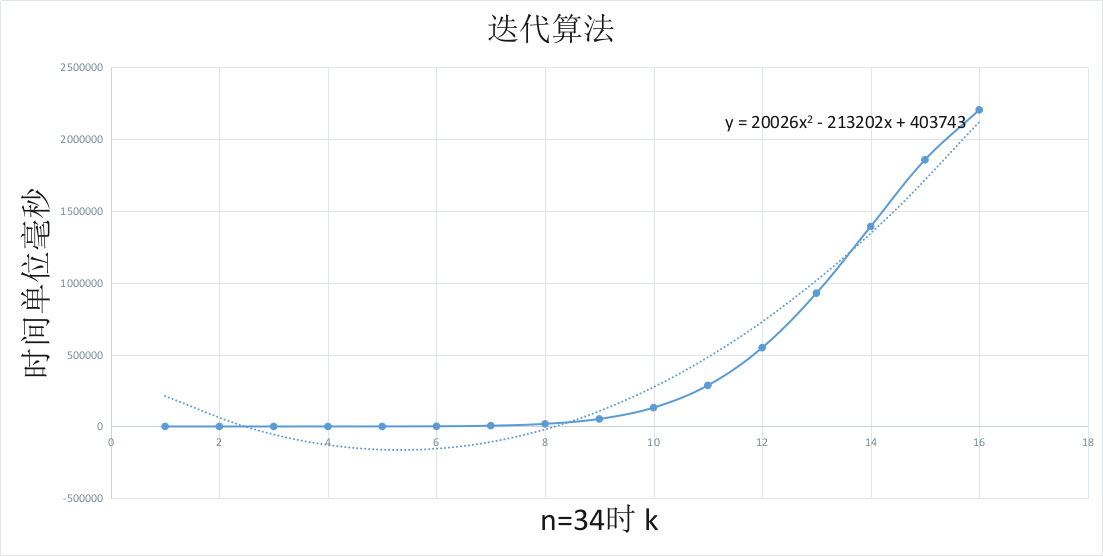
\includegraphics[scale=0.5]{../images/recursion.png}
	\caption{递归算法}
\end{figure}

\begin{figure}[H]
	\centering
	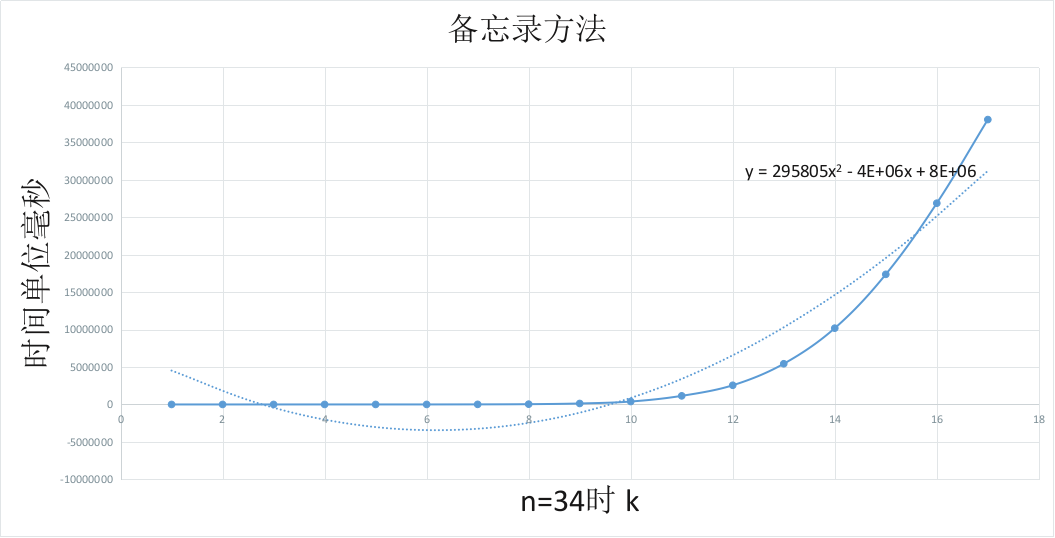
\includegraphics[scale=0.5]{../images/memo.png}
	\caption{备忘录方法}
\end{figure}

\begin{figure}[H]
	\centering
	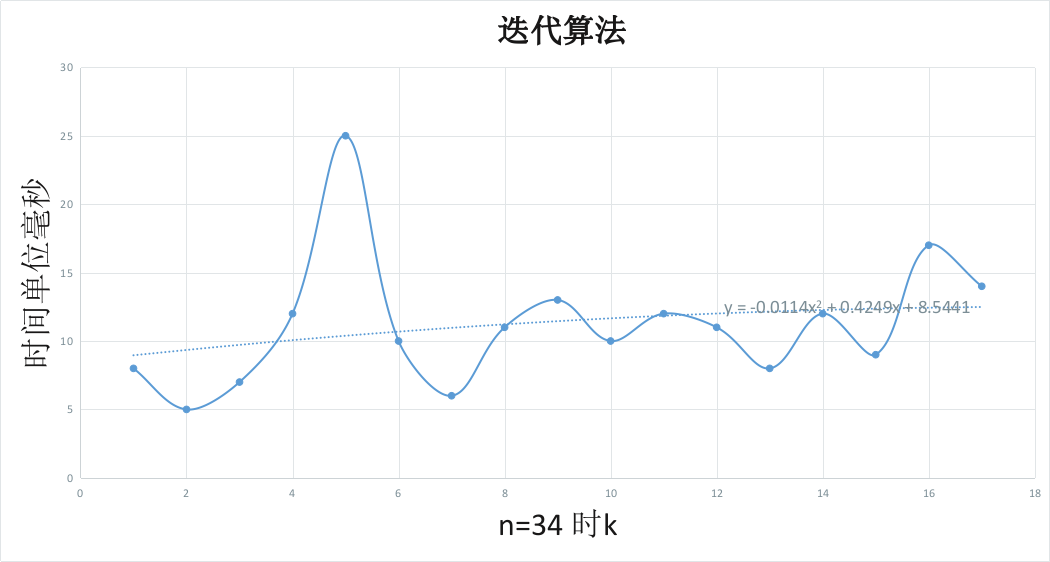
\includegraphics[scale=0.4]{../images/iteration.png}
	\caption{迭代算法}
\end{figure}

通过分析,可以得出{\bfseries 递归算法}的时间复杂度 $\Theta(n) = n^2$,空间复杂度为 $n^2$ ;{\bfseries 备忘录方法}的时间复杂度 $\Theta(n) = n^2,$空间复杂度为 $n^2$ ;{\bfseries 迭代算法}的时间复杂度 $\Theta(n) = n^2$,空间复杂度为 $n^2$ 。
\subsubsection{算法实例}
输入:$n=16, k=7$ 

输出:

\begin{figure}[H]
	\centering
	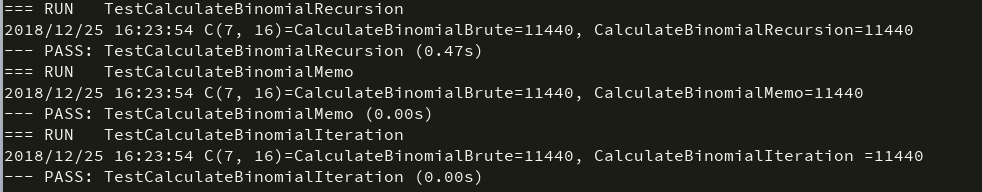
\includegraphics[scale=0.5]{../images/binomial-test.png}
	\caption{测试计算二项式的算法}
\end{figure}

\newpage
\subsection{绘制简单的分形树}
\subsubsection{问题描述}
\subsubsection{解决问题所用的算法设计方法及基本思想}
\subsubsection{采用的数据结构描述}
\subsubsection{算法描述 }
\subsubsection{算法的时间空间复杂度分析 }
\subsubsection{算法实例}

\newpage
\section{遍历}
\subsection{8品脱问题}
\subsubsection{问题描述}
\subsubsection{解决问题所用的算法设计方法及基本思想}
\subsubsection{采用的数据结构描述}
\subsubsection{算法描述 }
\subsubsection{算法的时间空间复杂度分析 }
\subsubsection{算法实例}

\newpage
\subsection{24点问题}
\subsubsection{问题描述}
\subsubsection{解决问题所用的算法设计方法及基本思想}
\subsubsection{采用的数据结构描述}
\subsubsection{算法描述 }
\subsubsection{算法的时间空间复杂度分析 }
\subsubsection{算法实例}


\newpage
\section{动态规划}
\subsection{最长回文子序列问题}
\subsubsection{问题描述}
\subsubsection{解决问题所用的算法设计方法及基本思想}
\subsubsection{采用的数据结构描述}
\subsubsection{算法描述 }
\subsubsection{算法的时间空间复杂度分析 }
\subsubsection{算法实例}


\newpage
\subsection{小美购物问题}
\subsubsection{问题描述}
\subsubsection{解决问题所用的算法设计方法及基本思想}
\subsubsection{采用的数据结构描述}
\subsubsection{算法描述 }
\subsubsection{算法的时间空间复杂度分析 }
\subsubsection{算法实例}

\newpage
\section{分支限界与回溯}
\subsection{n个处理机和k个任务问题}
\subsubsection{问题描述}
\subsubsection{解决问题所用的算法设计方法及基本思想}
\subsubsection{采用的数据结构描述}
\subsubsection{算法描述 }
\subsubsection{算法的时间空间复杂度分析 }
\subsubsection{算法实例}

\newpage
\section{附加题目}
\subsection{学习超市选址问题}
\subsubsection{问题描述}
\subsubsection{解决问题所用的算法设计方法及基本思想}
\subsubsection{采用的数据结构描述}
\subsubsection{算法描述 }
\subsubsection{算法的时间空间复杂度分析 }
\subsubsection{算法实例}

\section{课程设计总结}

\end{document}
